% Yes, this requires flipping flags to compile for different conferences...
% But you can press Ctrl+T while editing in TeXworks without having to change windows!

% conditional compilation
\def\buildemnlp{0}
\def\buildamta{1}
\def\buildhcomp{2}
\def\buildtarget{\buildamta} % required to be a single character for \if

\title{Return of the Linguist:\\Toward scalable parallel corpus generation for machine translation}

% emnlp2016.sty, included by header-emnlp.tex, does NOT tolerate ANY surrounding \else statements...
% an if/else if/... or ifcase statement would have been preferred...
% but \documentclass is declared in the header file, which results in some hidden error-checking:
    % unsupported \buildtarget will fail to build (``\usepackage before \documentclass'')
    % duplicate target values (e.g., emnlp=amta=0) will fail to build (``two \documentclass commands'')
\if \buildtarget \buildemnlp    
    % preamble from emnlp2016.tex to allow reuse of paper.tex between conferences

\documentclass[11pt,letterpaper]{article}
\usepackage{emnlp2016}
\usepackage{times}
\usepackage{latexsym}

% Uncomment this line for the final submission:
%\emnlpfinalcopy

%  Enter the EMNLP Paper ID here:
\def\emnlppaperid{137}

% To expand the titlebox for more authors, uncomment
% below and set accordingly.
% \addtolength\titlebox{.5in}    

\newcommand\BibTeX{B{\sc ib}\TeX}

%\title{Return of the Linguist:\\Toward scalable parallel corpus generation for machine translation}
%% according to my notes, I came up with this title around 3/11/16

% Author information can be set in various styles:
% For several authors from the same institution:
% \author{Author 1 \and ... \and Author n \\
%         Address line \\ ... \\ Address line}
% if the names do not fit well on one line use
%         Author 1 \\ {\bf Author 2} \\ ... \\ {\bf Author n} \\
% For authors from different institutions:
% \author{Author 1 \\ Address line \\  ... \\ Address line
%         \And  ... \And
%         Author n \\ Address line \\ ... \\ Address line}
% To start a seperate ``row'' of authors use \AND, as in
% \author{Author 1 \\ Address line \\  ... \\ Address line
%         \AND
%         Author 2 \\ Address line \\ ... \\ Address line \And
%         Author 3 \\ Address line \\ ... \\ Address line}
% If the title and author information does not fit in the area allocated,
% place \setlength\titlebox{<new height>} right after
% at the top, where <new height> can be something larger than 2.25in
%\author{Siddharth Patwardhan \and Daniele Pighin\\
%  {\tt publication@emnlp2016.net}}

\date{}

%%%\begin{document}

%%%\maketitle


    \newcommand\mycitep[1]{\cite{#1}}     % conference-specific ``glue code''
    \newcommand\mynewcite[1]{\newcite{#1}}
    \newcommand\amtaonly[1]{} % currently being used to trim down to 4 pages
    \newcommand\emnlponly[1]{#1}
    \newcommand\hcomponly[1]{}
\fi
\if \buildtarget \buildamta    
    % preamble from amta2016.tex to allow reuse of paper.tex between conferences

\documentclass[]{article}
\usepackage[letterpaper]{geometry}
\usepackage{amta2016}
\usepackage{times}
\usepackage{url}
\usepackage{latexsym}
\usepackage{natbib}
\usepackage{layout}

\newcommand{\confname}{AMTA 2016}
\newcommand{\website}{\protect\url{http://www.amtaweb.org/}}
\newcommand{\contactname}{research track co-chair Lane Schwartz}
\newcommand{\contactemail}{lanes@illinois.edu} 
\newcommand{\conffilename}{amta2016}
\newcommand{\downloadsite}{\protect\url{http://www.amtaweb.org/}}
\newcommand{\paperlength}{$12$ (twelve)}
\newcommand{\shortpaperlength}{$6$ (six)}

%% do not add any other page- or text-size instruction here

\parskip=0.00in

\begin{document}

% \mtsummitHeader{x}{x}{xxx-xxx}{2016}{45-character paper description goes here}{Author(s) initials and last name go here}
\title{\bf Formatting Your Paper \\
  for the \confname~Conference}  

\author{\name{\bf First Author} \hfill  \addr{author1@abc.university.country}\\ 
        \name{\bf Second Author} \hfill \addr{author2@abc.university.country}\\ 
        \addr{Department of Science, My University, 
        MyTown, Zip, Country}
\AND
       \name{\bf Third Author} \hfill \addr{author3@abc.university.country}\\
        \addr{Department of Science, My University, 
        MyTown, Zip, Country}
}

\maketitle
\pagestyle{empty}


    \newcommand\mycitep[1]{\citep{#1}} 
    \newcommand\mynewcite[1]{\cite{#1}}  
    \newcommand\amtaonly[1]{#1}
    \newcommand\emnlponly[1]{}
    \newcommand\hcomponly[1]{}
    
    % needed by Multeval tables
    \usepackage{amstext}
    \usepackage{multirow}
    
    \usepackage{graphicx}
    %\usepackage{caption}
    %\usepackage{subcaption}

\fi
\if \buildtarget \buildhcomp    
    \def\year{2016}\relax
%File: formatting-instruction.tex
\documentclass[letterpaper]{article}
\usepackage{aaai16}
\usepackage{times}
\usepackage{helvet}
\usepackage{courier}
\frenchspacing
\setlength{\pdfpagewidth}{8.5in}
\setlength{\pdfpageheight}{11in}
\pdfinfo{
/Title (Insert Your Title Here)
/Author (Put All Your Authors Here, Separated by Commas)}
\setcounter{secnumdepth}{2}  % 0-no numbers, 1-section numbers, 2-section and subsection numbers
% \begin{document}
% The file aaai.sty is the style file for AAAI Press 
% proceedings, working notes, and technical reports.
%
\title{Formatting Instructions \\for Authors Using \LaTeX{}}
\author{AAAI Press\\
Association for the Advancement of Artificial Intelligence\\
2275 East Bayshore Road, Suite 160\\
Palo Alto, California 94303\\
}
    \newcommand\mycitep[1]{\cite{#1}} 
    \newcommand\mynewcite[1]{\citeauthor{#1}~\shortcite{#1}}  
    \newcommand\amtaonly[1]{}
    \newcommand\emnlponly[1]{}
    \newcommand\hcomponly[1]{#1}
\fi
    
% Add support for snippets of \zh{中文}
\usepackage{CJK}
\usepackage[utf8]{inputenc}
\newcommand\zh[1]{\begin{CJK}{UTF8}{gbsn}#1\end{CJK}}

% this would allow clickable urls for my convenience - but many conferences forbid them?
% \usepackage{hyperref}



\begin{document}
\maketitle




% website limits abstract to 300-word, but that's WAY too long. Mine is about 70 words, and it's short but not too short.
\begin{abstract}
The large-scale generation of synthetic parallel corpora for data-driven machine translation is proposed\amtaonly{ in this demo paper}.
A rudimentary system for doing this is presented, with mechanisms for syntactic complexity in the spirit of classical rule-based machine translation and high-quality sentence pairs in the spirit of example-based machine translation.
Preliminary experiments integrating these synthetic corpora into a shared task are reported.
Promising future directions are discussed, in particular, large-scale contributions from ``amateur linguists'' via crowdsourcing.
\end{abstract}



\section{Motivation} 

As early as Jelinek's (in)famous quote during the 1980's that ``{\em Every time I fire a linguist, my performance goes up},'' both linguists and linguistics have been increasingly marginalized in natural language processing (NLP). 
More recently, for example, \mynewcite{collobert:2011} mention the possibility ``{\em [ideally]...to learn from letter sequences rather than words},'' illustrating an AI-motivated desire to move away from even fundamental linguistic concepts.
A specific instance of this overall trend is the gradual shift of machine translation (MT) away from classical linguistic rule-based approaches to contemporary machine learning approaches \mycitep{hutchins:2005}, which underlie statistical phrase-based systems like Moses \mycitep{moses} and more recent neural network systems \mycitep{sutskever:2014,bengio:2014}.  
But in the end, even the most cutting-edge machine learning MT system relies crucially on bilingual parallel corpora, typically taken from external sources like multilingual parliamentary proceedings. 
This results in what we perceive to be a disproportionate amount of effort being dedicated to the machine learning component of machine translation, with input corpora being treated almost as an afterthought.\footnote{
    Of course, these parallel corpora represent hundreds of translator-hours of work. 
    However, such translations are optimized for human consumption, not machine learning, with no regard for such niceties as sentence alignment.
    \amtaonly{
        This is not unlike an athlete having an Olympic-level training regimen, fueled by food scrounged off the streets.
        
        An example of suboptimal parallel corpora being used for machine translation is given in Section \ref{subsec:case_study}.
        At the very least, it suggests a need for more careful post-editing of bitexts, particularly for development and test corpora.
        More ideal, though, would be the creation of parallel corpora for the express purpose of training, tuning, and evaluating data-driven MT systems.
    }    
} % footnote
% TODO: modernization of corpus acquisition / bring machine learning to bear here too
    
% it's TEMPTING to say this, but the same is essentially true of all supervised data sets - they're pretty much all human-labeled...
%It is surprising to say the least to contrast 
%technological sophistication
%
%with the direct human translation 
%whereas parallel corpus acquisition is still more or less entirely dependent on .



One of the major advantages of data-driven MT is that it removes the need for linguists to develop a new set of rules for an MT system to support a new language.
In a sense, though, the rule-based MT linguist's job has really been  ``outsourced'' to third-party translators, who implicitly encode linguistic information in parallel corpora.
We believe there is still a significant ``in-house'' role for linguists to play in corpus-based machine translation, and that is to direct the crafting of high-quality, ``designer'' synthetic parallel corpora, leveraging technologies like crowdsourcing to maximize throughput.
Such a division of labor would let linguists be linguists, with MT system development proceeding in parallel.  
% TODO: let machines be machines, do what machines do best


%\amtaonly{\subsection{Potential Benefits}}
\label{subsec:benefits} % ha, this works even if it's not a subsection - LaTeX just figures out what sec/subsec it's in

Large, high-quality synthetic parallel corpora could be useful as:

\begin{itemize}
\item Training sets for corpus-based MT systems, particularly for low-resource language pairs
\item Benchmark tasks for MT evaluation, in the spirit of Facebook's bAbI project \mycitep{bAbI}
\item Translation memories for computer-assisted translation
\item ``Language archives'': New NLP methods are developed every few years; linguistic theories change every decade or so; parallel corpora live forever (like the Rosetta Stone).
\end{itemize}
% sigh, this set of bullets seems much clearer than all those stupid sentences that came before

We believe that natural language processing in general and machine translation in particular are particularly amenable to artifical data generation. 
Unlike many machine learning applications (image recognition, finance), NLP data sets are manmade to begin with; humans themselves {\em are} the primary natural producers and consumers of raw written language data.
Translation is further privileged as perhaps the only NLP task for which millions of people (foreign-language learners) already undergo years of formal training, which has implications for scalability via crowdsourcing (Section \ref{sec:future}).

% TODO: corpus generation is (almost like?) a sub-problem
% TODO: a reference to ``blessing of dimensionality'' for the inverse problem? how it's relatively easy to generate an exponentially large number of sentences?
% TODO: tree-based methods become a lot easier too? I even construct a random stupid tree myself...
Other practical considerations shine a favorable light on parallel corpus generation.
As the ``inverse'' of translation, multilingual generation is also an easier task in some senses.
For example, lexical ambiguity can be largely alleviated,\footnote{
    Ideally the generator would ``know'' {\em a priori} whether it is writing a sentence about, say, (financial) banks or (river) banks.
} segmentation of languages like Chinese \mycitep{segmenter:2008} becomes a non-issue, and there is the potential for generating annotated corpora with zero annotation error.
In principle, high-quality alignments could be obtained at the word or phrase level for use in the statistical MT process, and these alignments 
could also be potentially useful in training methods for MT subtasks such as syntactic pre-reordering \mycitep{prereordering}.
Parallel corpora also provide a natural avenue to interface contemporary MT systems with the countless linguist-years of expertise that have been invested into rule-based MT systems. %, as discussed in Section \ref{sec:related}. % that's not really discussed there anymore, is it?
And unlike the various different MT methods, which are by nature competitive, corpora are inherently collaborative.

This paper is organized as follows.
Section \ref{sec:related} discusses previous related work,
Section \ref{sec:generator} describes our rudimentary parallel corpus generator,
Section \ref{sec:experiments} gives experimental results, 
and Section \ref{sec:future} proposes future work.



\section{Related Work}
\label{sec:related}

The idea of using synthetic parallel corpora in machine translation is hardly new.
% TODO: it's not domain limitation that matters - it's the fact that they're not amplifying, just mapping sentences 1-1
Previous attempts at creating synthetic parallel corpora have used rule-based MT (RBMT) systems \mycitep{hu:2007,dugast:2008,murakami:2009,rubino:2014}, but the input to the RBMT systems was again dictated by external corpora in the desire to produce immediate results.
A longer-term approach that may pay dividends (Section \ref{subsec:benefits}) would be to run RBMT systems on specially chosen sentences for which they are known to produce high-quality translations, or perhaps eventually directly encoding their rules into carefully crafted parallel corpora.

Our parallel corpus generation system (Section \ref{sec:generator}) is very similar to the recursive equivalence class approach to example-based MT \mycitep{ebmtbook} used by \mynewcite{brown:99}. 
Our generator has more of a rule-based flavor, using a somewhat more varied grammar that also admits the use of participial noun modifiers.
But more importantly, we believe this line of work was ahead of its time and consider our main contribution to be bringing attention to its potential value to contemporary MT.  

Equivalence classing is in fact an integral part of the standard pipeline of Moses \mycitep{moses}, the open-source statistical MT system. 
During training, the {\small \tt mkcls} component adds ``{\em an `example-based' touch to the statistical approach}'' by clustering words into automatically-generated equivalence classes to ameliorate data sparsity issues \mycitep{och:98}.
However, these clusters are trained only at the word level and not for phrases, and the clusters themselves are typically only used during alignment.
Furthermore, since they are learned in an unsupervised manner from the parallel corpus, they can still benefit from the addition of more high-quality training examples, synthetic or otherwise.

% POTENTIAL REVIEWER QUESTION (assuming they even understand wtf I was talking about here): well, but you can add word cluster ids as factors/features... (http://www.statmt.org/moses/?n=Advanced.Models#ntoc6 - simply annotate words )
% my weak responses
    % supervised data almost always trumps unsupervised data, especially in NLP. there is no real substitute for REAL, in-domain data
    % also, you would still have to require the models to to learn from these noisy clusterings
    % actually, word+mkcls is still a LEXICALIZED translation factor; that's probably why it doesn't really help during the translation phase
        % class-LM (target sequence model over cluster-ids) seems like it might be more useful....BUT, this is for MONOLINGUAL target-side data, 
            % which generally doesn't need the help
            % which is a strange thing to do to begin with, taking clusterings that were trained on expensive bilingual corpora and using them on plentiful monolingual corpora
% a possibly stronger response: automatic clusters are also of lower quality than hand-crafted template variations, and there will likely be clustering errors
% side note: if mkcls clusters were so awesome, they'd be used as standard factors... so you'd have to think that they're not
% TODO: propose ``next-generation mkcls''? meh that's so ridiculously vague...

% these links are too long for EMNLP. TODO: add them as footnotes for AMTA?
% 

In terms of freely available multilingual natural language generators, the most well-developed one we found was KPML \mycitep{kpml}.
But crafting sentences using KPML is a lengthy process,\amtaonly{\footnote{
    For examples, see http://www.fb10.uni-bremen.de/anglistik/langpro/kpml/genbank/generation-bank.html}} involving a well-developed linguistic theory to explain the surface forms.
In contrast, our primary goal is to generate large parallel corpora of surface forms quickly. 
% This affords us an amount of flexibility as to the method of generation. % redundant and doesn't really flow
% TODO: for our purposes, the linguistic correctness of a generator (hokey hidden structures) is less important than whether it generates well-translated sentences.

In the next section, we describe our own primitive attempt at building a multilingual generator from scratch. 
While we try to model straightforward linguistic phenomena compositionally, we also adopt the pragmatic attitude, in the tradition of example-based MT \mycitep{ebmtbook}, that sometimes the most effective way to represent a translation phenomenon is simply to write it down.
Thus, with the long-term goal of scalability, we attempt to construct a system sufficiently flexible to write some sentence pairs in large quantities through syntactic variations and others with ``hand-crafted'' quality through example-based templates.


\section{A Rudimentary Multilingual Generator}
\label{sec:generator}

% TODO: didn't mention how you could easily create infinitely many sentences like ``the number of cats is N'', but they'll be soo correlated that they have zero translation value



As an example of how our synthetic parallel corpus generation system works, consider the following English-Chinese template pair:

%\small
\begin{center} \begin{small} 
{\tt S V O .} \\
{\tt S \zh{把} O V \zh{。}}
\end{small} \end{center} 
%\normalsize

\noindent Our system then expands the subject {\small \tt S} and object {\small \tt O} as noun phrases, adding adjectival and participial modifiers as desired. 
Semantic constraints can be imposed from the verb {\small \tt V} as well as externally.
The generator can then vary the template lexically and syntactically,\footnote{\label{footnote:probabilities}
    Rewrite probabilities were set by hand; a more principled approach might use, say, a generative synchronous CFG.} allowing a large number of sentence pairs to be generated from a single template.
We can also trade quantity for quality by adding more literals to the template, in the spirit of example-based MT.




%This Section is organized as follows. 
%Section~\ref{subsec:software}, we describe our software architecture and internal data representation. 
%Section~\ref{subsec:linguistics} then covers the linguistic phenomena we implemented in this framework.

% TODO: maybe these nonsense sentences shed some light as to what is NOT a sensible, ``natural'' sentence...
\amtaonly{
\subsection{Simplistic Linguistics}
\label{subsec:linguistics}
}
We adopt an extremely simplistic view of language as nouns, verbs, and their modifications and elaborations.
\amtaonly{
Inspired by early work on transformations by \mynewcite{chomsky}, we focus on declarative indicative present active sentences in the hopes that they can be transformed into other forms in the long run. 
Similarly, although we enforce some semantic constraints, our system generally produces nonsensical sentences like Chomsky's celebrated ``{\em Colorless green ideas sleep furiously.}''
}The fact that verb phrases can also serve as nouns (gerundives) and modifiers (participles) appears to be a major source of syntactic complexity, and we made it a priority to implement participial modifiers.

\amtaonly{

\subsection{Software Architecture}
\label{subsec:software}


The bulk of our software, which we plan on eventually open-sourcing, along with its accompanying data, comprises four Python modules:\footnote{
    In particular, we used Python 3 for its improved Unicode support over Python 2.
}

\begin{itemize}
\item {\small \tt data}: data abstraction layer
\item {\small \tt nodes}: internal tree representation
\item {\small \tt generator}: converts internal trees to surface forms (sentence pairs)
\item {\small \tt main}: outermost logic
\end{itemize}

The {\small \tt data} module implements an abstraction layer that mediates between data resources on disk and the rest of the program.
These data resources include bilingual (extensible to multilingual) lexicons for different parts of speech, monolingual morphology, templates, and a small taxonomy used to tag nouns.
All of our data resources were written in YAML, a ``human-readable'' language particularly well-suited to manual editing.
In particular, YAML has native Unicode support and does not even require quotation marks to enclose strings.
An example of YAML code is shown in Figure~\ref{fig:yaml-rb}.

% TODO: probably going to have to resize/crop this image to keep this paper from going over length
% TODO: YAML code examples. couldn't get verbatim + zh to work... just use an image? see if there's room.
% TODO: manually indent YAML. use placeholder graphic for now instead.
% TODO: get proper left/right subfigures working? just slapping in a single image for now.
\begin{figure}[ht]
    \centering
    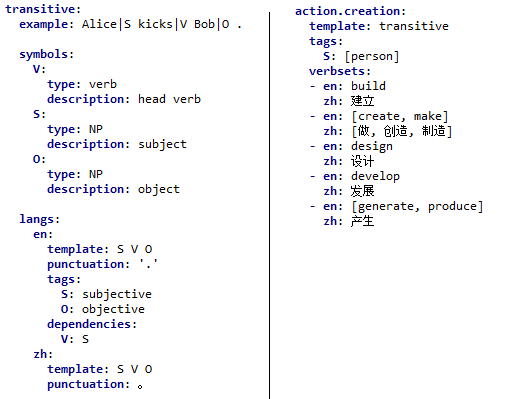
\includegraphics{yaml-rb}
    \caption{An example of YAML code, showing syntactic (left) and semantic (right) components of a clause template used for the ``rule-based'' mode of generation mentioned in the discussion of the {\small \tt main} module.}
    \label{fig:yaml-rb}
\end{figure}
 

% the internal data representation. the bulk of the discussion?
The {\small \tt nodes} module implements the data structures used internally by the program.
To capture recursive structures like participles, we adopt a rudimentary tree representation that is something intermediate between constituency and dependency trees, with constituent-like modifiers that also maintain dependency-like links to their targets.
Following our highly simplified picture of linguistics in Section~\ref{subsec:linguistics}, the basic backbone of the tree is constituency-like, as shown in Figure~\ref{fig:tree}.

% TODO: nodes class diagram? seems like an implementation detail...
% TODO: the fastest way i have to get dotted lines is through Word or PowerPoint, but I wanted to do the figures in OneNote, at least the camera-unready ones...
% TODO: it would be NICE if the tree matched a YAML example...
\begin{figure}[ht]
    \centering
    placeholder graphic, used to estimate space remaining in the paper
    \includegraphics{yaml-rb-rotated}
        
    \caption{
        An example tree made of nodes from the {\small \tt nodes} module.
        Thick lines indicate the ``constituent'' backbone that dictates the order of traversal in the {\small \tt generator} module, while thin lines indicate longer-range dependencies that are stored as links between nodes.
    }
    \label{fig:tree}

\end{figure}
    


% TODO: class hierarchy for nodes module only??
% - data is too mundane, and i'll just describe it in words.
% - Generator is only 2 classes, and i'll also just describe it in words.
%- ad hoc semantic taxonomy that allows a template to request


The {\small \tt generator} module traverses the backbone of the ``interlingual'' tree from the {\small \tt nodes} module and recursively builds up parallel surface forms (bilingual sentence pairs).
Language-specific rules (e.g., word order) are implemented as ad hoc bits of code in this module,\footnote{
    Formally, the ``rule-based'' component of our system can be considered an extremely rudimentary synchronous (bilingual) context-free grammar of sorts \mycitep{transduction} that also admits long-range dependencies and semantic constraints.
    But it would be a disservice to those other well-developed methods to refer to our system as anything other than an ad hoc way to generate multilingual sentences.
%    MEH: Also, example-based mode admits the possibility of just writing down translations and then generating parse trees on PORTIONS of those templates.
%    Although then I guess you have a transductive grammar on those portions?
} reading long-range dependency information from the tree as needed.
All language-dependent code is confined to this module, although this is coupled with language-dependent information from the YAML data (e.g., the tags and punctuation in Figure~\ref{fig:yaml-rb}). 
% TODO: More ideally, A desirable longer-term goal would be to move language rules to data, but that's beyond the scope of this paper.


Finally, the outermost {\small \tt main} module is responsible for tree instantiation and modification.
To generate a sentence pair in ``rule-based mode,'' a syntactic clause template is randomly selected, followed by a semantic verb category that uses that syntactic template, as in Figure~\ref{fig:yaml-rb}.
Modifier nodes are then randomly attached, recursively so for constructs like participles and prepositions, in principle admitting arbitrarily long sentences.
The probabilities for these random processes are chosen heuristically as mentioned in Footnote~\ref{footnote:probabilities}.
The system also allows for semantic constraints by adding semantic tags to nodes and querying the taxonomy through the {\small \tt data} module for eligible lexical choices. 
%For example, the semantic template component in Figure~\ref{fig:yaml-rb} requires a person for the subject node, and it should be able to query the noun database for UGH
Building a comprehensive taxonomy and labeling the lexical database exhaustively is a labor-intensive task; results in Section~\ref{supersec:experimental_results} below were obtained with relatively minimal semantic constraints.


% example-based amplification: loop over different lexical choices exhaustively
One of the things we wanted to do differently from KPML \mycitep{kpml} was to implement an ``example-based mode'' in which sentence pairs that would be difficult to generate in ``rule-based mode'' could simply be written down and then amplified as proposed by \mynewcite{brown:99}. 
This would trade the quantity available through arbitrarily complex sentences from ``rule-based'' mode for the quality of sentence pairs with a larger degree of hand-translation.
Our software achieves this by allowing the {\small \tt template} entries as on the left side of Figure~\ref{fig:yaml-rb} to contain literal strings in addition to symbols.
These ``example-based'' templates are currently selected by hand for the experiments described in Section~\ref{supersec:experimental_results}, with all amplification resulting from varying the lexical choices (i.e., without adding ).
Whether it helps to add modifier nodes in this mode is a potential area for future work.
% TODO: meta-template picture (if space allows)? or is this description adequate? this is kind of like the tradeoff I faced in the EMNLP submission, where I was like, uh oh, out of space... meh, this system sucks anyways, so I'll just omit its details
A helper script also supports the use of ``meta-templates'' to facilitate hand-construction of templates, allowing a minimal annotation of a sentence pair to produce a full YAML template similar to Figure~\ref{fig:yaml-rb}.

%% TODO: ugh, out of room? this stuff is pretty pointless anyway
%It is hoped that these ``example-based'' templates prove useful for tasks like training set amplification, which we consider in Sections~\ref{sec:experiments}~and~\ref{subsec:post_edited}. 
%But it would be very easy to specify modifiable nodes in the meta-templates, and you could add modifiers as in ``rule-based'' mode.
%The point of rule-based templates (and indeed linguistics) is to be precise and write a few rules that can generate a lot of sentences.
%But for example-based templates, we want to do lots of sentences, fast, and then maybe amplify little pieces of it.
%Meta-templates let you iterate quickly over sentences.

%An example of such a meta-template is given in Figure~XXX, which corresponds to the example-based template given above in Figure~YYY
%\begin{small}
%\noindent {\tt S V O .} \\
%{\tt S \zh{把} O V \zh{。}}
%\end{small}


% figure: example-based template, and its associated 
%meta-templates, which can then be easily parsed into templates to be fed into the generator.
% one big image, top/bottom?
%An example is shown in Figure~\ref{fig:yaml_template}.





%} \hcomponly{ % disable last bit of unfinished stuff for temp upload


%%%%%%%%%%%%%%%%%%%%%%%%%%%%%%%%%%%%%%%%%%%%%%%%%%%%%%%%%%%%%%%%%%%%%%%%%%%%%%%%%%%%%%%%%%%%
\noindent\makebox[\linewidth]{\rule{\paperwidth}{0.4pt}} % full-width horizontal line
TODO

\subsection{Implemented Linguistic Phenomena}

We briefly list
and how they are implemented in terms of the tree representation from Section~\ref{subsec:software}

a couple of reasons for keeping linguistic phenomena to the most basic ones (aside from manageability)
- we believe that for the purposes of generating parallel corpora, is most effective to treat very difficult, non-compositional phenomena (example?!) by simply writing them down, in tradition of example-based MT
- keeping the data format simpler makes it potentially easier to scale up to admit contributions from non-linguists

- emphasize that we prioritize generating in-domain sentences above linguistic soundness

% transformations were chosen with an eye toward scalability, so that things like semantic constraints (<animal> eats <food>) could be used (eating <food>, and should modify <animal>)

% if i'm gonna do source code snippets with zh, maybe it'd be best to use IMAGES? it's not for camera-ready anyway...
% well, i can do the meta-template easily... the problem is with REAL templates

% maybe use a bulleted list for the different linguistic phenomena supported? yeah, let's just do that.

%Oh, maybe I should make this a table. that should cut down on the vertical spacing
%
%\begin{table}[ht]
%\centering
%\begin{tabular}{|l|l|}
%\hline
%Gold en & 60,000. \\ \hline
%Gold en & 60,000. \\ \hline
%Gold en & 60,000. \\ \hline
%Gold en & 60,000. \\ \hline
%Gold en & 60,000. \\ \hline
%Gold en & 60,000. \\ \hline
%Gold en & 60,000. \\ \hline
%Gold en & 60,000. \\ \hline
%Gold en & 60,000. \\ \hline
%Gold en & 60,000. \\ \hline
%\end{tabular}
%\caption{ 
%    Linguistic constructs implemented in our multilingual generator.
%}
%\label{tab:implemented_linguistics}
%\end{table}

\begin{itemize}
\item clauses: transitive, meta, modal. a word on modalish. 
\item NP
\item ADJP
\item participles as transformations of clauses that convert subject into a linked node, allowing reuse of semantic constraints
\item prepositions as relations between two nodes (noun/noun or noun/verb), and accompanying semantic requirements on both object and target
\item custom nodes - because sometimes, the most effective way to represent a translation is to just write it down. (``template-based mode''): lots of iterals, maybe mark an NP somewhere

% other (if there's room)
\item ADVP (targeting ADJP or Clause), pronouns with antecedents 
\item indirect object as a special case of ``null preposition'' - not necessarily linguistically well-founded, but good enough to make sentences
\item past tense as transformation of present tense  % MEH
\item other transformations: topicalization, and some hokier stuff like \zh{把} 
\end{itemize}



% big question: do I want to show a source code example?? yeah, i probably have room
\noindent\makebox[\linewidth]{\rule{\paperwidth}{0.4pt}} % full-width horizontal line
%%%%%%%%%%%%%%%%%%%%%%%%%%%%%%%%%%%%%%%%%%%%%%%%%%%%%%%%%%%%%%%%%%%%%%%%%%%%%%%%%%%%%%%%%%%%
} % amtaonly







% oh this part really is just flying now, because there's no uncertainty as to what I DID



\section{Experimental Results}
\label{supersec:experimental_results}

%\subsection{Methods} % no space? just do one paragraph each?
\amtaonly{\subsection{Training Set Amplification}}
\label{sec:experiments}
We now consider training set amplification as a first application, using the Chinese to English MT task of IWSLT 2015 \mycitep{iwslt2015}\emnlponly{.}\amtaonly{, mentioned briefly in Section \ref{subsec:case_study}.}
This task uses the WIT$^3$ corpus \mycitep{wit3}, which consists of multilingual subtitles of TED talks covering a wide variety of subjects. 
The freely available MultiUN corpus \mycitep{multiun} from the OPUS project \mycitep{opus:2012} was also used for comparison.

To investigate the relative effect of our synthetic parallel corpora, we chose a simple baseline system and fixed all other variables.
Namely, we used the baseline configuration of Moses \mycitep{moses} as described in \mycitep{iwslt2015}, with the exception of changing the target language model to KenLM \mycitep{kenlm}, which we found to be faster and stabler at decoding time than IRSTLM \mycitep{irstlm}.
Since monolingual corpora are typically available at scale, target language models were obtained using the same in-domain monolingual corpus for all runs.
For the remaining unspecified model settings, we used the {\small \tt grow-diag} alignment heuristic recommended by \mynewcite{segmenter:2008} and the {\small \tt mslr-fe} configuration for lexicalized reordering. 
Chinese text was preprocessed using the latest version of the Stanford Segmenter \mycitep{segmenter:2008}.
Phrase and lexicalized reordering tables were interpolated using the {\small \tt tmcombine} script included with Moses \mycitep{tmcombine}, with the interpolation optimized on the {\small \tt dev2010} data set.
Following \mynewcite{iwslt2015}, the model was tuned on the {\small \tt tst2010} data set using the MERT procedure included in Moses.
For Table~\ref{tab:results}, BLEU scores were computed as described by \mynewcite{iwslt2015} using the IWSLT 2015 progress data set ({\small \tt tst2014}).\footnote{
    We chose the {\small \tt tst2014} test set to facilitate comparison with published results from both IWSLT 2014 and 2015 in future work.
} % might be nice to throw this sentence into the Table caption, but LATeX chokes on the \footnote{}

% TODO: propose using sub-sentence timing information? you already HAVE relatively fine-grained alignment information... but the corpus crawler just throws that away. Then again, you might get stuff like cross-fragment alignments...

% TODO: add OpenSubtitles 2016 results? they don't really add much to the discussion - I can just mention them briefly, maybe even in a footnote
% oh okay, this is nice - if I don't include OpenSubtitles, then I don't have to talk about the stupid purging either
%heuristically purged zh\_zh, which is a very noisy corpus
%zh\_zh corpus from the OpenSubtitles 2016 corpus , with lines cleaned using some ad hoc heuristics


% side-by-side tables as in emnlp2016.tex
\begin{table}[ht] % h for ``here'' - float the table right here in the text, instead of at the top of page
\centering
\small
\begin{tabular}{cc}

\begin{tabular}{|l|r|}
\hline
                    & BLEU   \\ \hline
25\% corpus         &  9.95  \\ \hline
  + 75\%            & \textbf{11.47}  \\ \hline
  + MultiUN         & 10.76  \\ \hline
  + Generated       &  9.91  \\ \hline
\end{tabular}

\begin{tabular}{|l|r|}
\hline                    & BLEU   \\ \hline
Official            & 11.43  \\ \hline
Our baseline        & 11.54  \\ \hline
  + MultiUN         & \textbf{11.67}  \\ \hline
  + Generated       & 11.46  \\ \hline
\end{tabular} & % oh this is how you get 2 tables side by side

\end{tabular} % cc (i.e., the big super-table)

% TODO: adding (fairly arbitrary) out-of-domain corpus is really more like using a different model (or maybe bagging?)

% TODO: mention that official results are on a slightly different Moses configuration? mehhhhh
\caption{ \label{tab:results} % oh, for reference numbering, label goes INSIDE caption
    (Left) Chinese-to-English BLEU scores for our baseline Moses configuration with phrase and reordering tables trained on a random 25\% subset of the IWSLT15 training corpus and interpolated (+) with tables for the remaining 75\% ($\sim$150K) of the in-domain corpus, the MultiUN corpus (a $\sim$1M line subset), and a synthetic corpus from our generator ($\sim$5M lines).
    (Right) Same as the left, but starting from tables trained on the entire IWSLT15 corpus.
    Official published scores of the IWSLT15 baseline system are also given for comparison.    
    Qualitatively similar trends for NIST and TER scores were also observed (omitted for clarity).
} % caption

\end{table}

% preemptively answering reviewer question: yeah yeah, the trained tmcombine weights are like 0.001 for my generated corpora
The results of these experiments are shown in Table~\ref{tab:results}.
For the table on the left, note that adding in-domain data improves performance significantly more than a much larger amount of out-of-domain data (MultiUN), a commonly reported phenomenon \mycitep{tmcombine}.
TED talks, which are prepared lectures, fall somewhere between the conversational language of movie subtitles and the formal written language of UN resolutions.
As such, the OpenSubtitles\footnote{http://www.opensubtitles.org/} 2016 corpus \emnlponly{\mycitep{opensubtitles:2016} }from the OPUS project was also out-of-domain; results for this corpus were similar to MultiUN and are not shown. % AMTA: removed citation to keep reference list under length
For the table on the right, note the diminishing returns of out-of-domain data as the amount of in-domain data increases.
These observations underscore the importance of domain overlap and hint at the potential value to be found in the amplification of in-domain corpora.

Our generated corpora do not yet make a significant impact on the final BLEU score,\footnote{
    The sub-baseline scores shown are for our most recently generated synthetic corpus; scores slightly higher than our baseline have also been obtained on older generated corpora.
    Both of these outcomes seem to be within experimental error bars.
}
indicating that our parallel corpus generator has a long way to go.
Development on our generator has so far focused on ``rule-based'' syntactic diversity and growing a lexical database tailored to the training set. 
Given the resulting scores, a change of direction seems in order; work on harvesting more ``example-based'' templates from the IWSLT15 training corpus is currently in progress.
\amtaonly{
As a first step in this direction, we examine the gold corpora qualitatively.}


% TODO: maybe add Bing and Google results, since nobody seems to report these? save this for AMTA? (haha not gonna have room, sucka)
% but should also add IWSLT-best results if you're doing that - and I don't see the point, unless my results were anywhere NEAR them
% nah, if at all, just mention in a table caption briefly somewhere



% new results for AMTA, and adding the old ``case study''
%%%%%%%%%%%%%%%%%%%%%%%%%%%%%%%%%%%%%

    
\amtaonly{ 
\subsection{Qualitative Analysis of Corpora}
\label{subsec:case_study}


Consider the official Chinese to English baseline translation of the {\small \tt tst2010} data set\footnote{
    \label{foot:tst2010}https://wit3.fbk.eu/score.php?release=2014-01
}.
As a crude way of assessing translation quality, we used the official evaluation software MultEval \mycitep{multeval} to compute scores for each translated line individually.
Upon manual inspection, the worst scoring individual lines (especially above 150\%) were almost all found to correspond to poor human translations on the Chinese side of the gold corpus.
This is particularly unsettling because the {\small \tt tst2010} data set has been used as the official development/tuning set for the past several IWSLT evaluation campaigns. 
The fact that these errors have persisted this long ({\small \tt tst2010} has been distributed with only minor changes for every IWSLT Chinese-English evaluation campaign since 2012) is a testament to how insidious these errors can be, even for a prominent international workshop. 



% TODO: display an example bad-sentence pair? If I don't, then what was the point of getting zh fonts working?? sigh

\begin{table}[ht]
\centering
\begin{tabular}{|l|l|}
\hline
Gold zh & \zh{安德森:是六万美元。} \\ \hline
Gold en & 60,000. \\ \hline
Moses output & CA : That is 60,000 dollars .  \\ \hline
\end{tabular}
\caption{ \label{tab:bad_pair}
   A ``poorly translated'' sentence pair from {\small \tt tst2010}, with a TER score of 250\%.    
}
\end{table}

An example is given in Table~\ref{tab:bad_pair}.
The baseline Moses system tries valiantly, but it ultimately scores poorly for producing a good machine translation of a liberal human translation.
Alternatively, one can interpret these errors as an additional source of noise in the human encoding of English into Chinese.
It is not immediately obvious how the MT process is affected by this kind of noise.

The most effective automated ways we found to identify lines in dire need of post-editing were:
\begin{itemize}
\item 
Duplicated Chinese segments on the same line. 
This was presumably caused by having the same sentence displayed at multiple time points in the video subtitles. 
Often, this would also indicate passages that were poorly aligned at the sentence level.
Such translations might suffice for viewing translated videos monolingually, but they are far from ideal for training a machine translation system.

\item 
Missing segments (usually English) when compared with the original lecture transcripts online.\footnote{http://www.ted.com/} 
This issue seems to have been introduced in the IWSLT15 Chinese-English corpus, and was also indicative of misaligned sentences.
%When applied to the IWSLT14 corpus, most of these would be ``false positives'' indicating post-editing of musical symbols and other artifacts.
%True positives were often indicative of misaligned sentences.
\end{itemize}



\subsection{Experiments on Post-Edited Corpora}
\label{subsec:post_edited}

% SLIGHTLY inconsistent formatting, since now I have discussion ABOVE the table instead of below...
% but this creates a natural break for the discussion 
Table~\ref{tab:tst2010} shows the scores obtained by ``lightly'' post-editing the MERT tuning set {\small \tt tst2010} as follows. 
On the Chinese side, duplicated segments, applause lines, and translator notes were removed. 
Speaker annotations were normalized on both sides, as well as sentence alignments wherever possible.
As a result, small but noticeable differences in scores are observed. 
(For comparison, the difference between the best and worst scoring Chinese-to-English systems in IWSLT14 \mycitep{iwslt2014} was 6 BLEU points and 7 TER points.)
In this case, the post-edited tuning set seems to guide the MERT optimization procedure of Moses to a slightly different local optimum.

% my baseline - 2016-05-15-213619
% tst2010 fixed lite - 2016-06-17-131927
\begin{table}[ht]
\centering
\begin{tabular}{|l|r|r|r|}
\hline
                    & BLEU  & NIST & TER    \\ \hline
(a) Official IWSLT15    & 11.43 & \textbf{4.67} & 72.65  \\ \hline
(b) Our baseline        & 11.54 & 4.43 & \textbf{72.43} \\ \hline
(c) Post-edited {\small \tt tst2010} & \textbf{11.91} & 4.33 & 75.34 \\ \hline
% &  &   \\ \hline
\end{tabular}
    % TODO: fairly labor intensive, not THAT much payoff? but there is definitely a payoff, and if you could crowd-lever it...

\caption{ \label{tab:tst2010}
    Chinese-to-English translation scores evaluated on the {\small \tt tst2014} data set, with experimental parameters as described in Section~\ref{sec:experiments}. 
    (a) Official published IWSLT15 baseline scores \mycitep{iwslt2015}, for comparison.
    (b) Our baseline Moses configuration, which uses KenLM instead of IRSTLM, as described previously.
    (c) Same as (b), but with a post-edited tuning set {\small \tt tst2010}. 
} % caption
\end{table}

For the rest of this section, we show the results of applying post-editing to corpora used for multiple purposes.
To preserve the integrity of {\small \tt tst2014}, evaluation is now performed using MultEval \mycitep{multeval} on the {\small \tt tst2010} data set itself, with the MERT procedure tuned on the {\small \tt dev2010} data set instead.
Our baseline model is also trained on the IWSLT corpus Chinese-English training corpus from 2014 instead of 2015.
These data sets and this evaluation software were used by the official WIT$^3$ benchmark linked in footnote \ref{foot:tst2010}.
MultEval has the added benefit of providing bootstrapped error bar estimates.

In tables with MultEval scores below, metric scores for all systems were generated using MultEval 0.5.1 \mycitep{multeval}: jBLEU V0.1.1 (an exact reimplementation of NIST's mteval-v13.pl without tokenization); Translation Error Rate (TER) V0.8.0. 
The $p$-values are relative to our baseline and indicate whether a difference of this magnitude (between the baseline and the system on that line) is likely to be generated again by some random process (a randomized optimizer). 
Metric scores are averages over three runs per system. 
$s_{sel}$ indicates the variance due to test set selection and has nothing to do with optimizer instability.\footnote{
    This paragraph and the tables with MultEval results are adopted from \LaTeX~code automatically generated by MultEval.
}





% TODO: didn't run MultiUN + tst2010 - but that's okay I guess, I have the out-of-domain in-domain comparison in Table 1

\begin{table}[htb]
\begin{center}
%\begin{footnotesize}
\begin{tabular}{|l|l|l|l|l|l|}
\hline
\bf Metric & \bf System & \bf Avg & \bf $\overline{s}_{\text{sel}}$ & \bf $s_{\text{Test}}$ & \bf $p$-value \\
\hline
\multirow{6}{*}{BLEU $\uparrow$}
& Official IWSLT14 baseline  & 11.2 & -   & -   & - \\
& Our baseline & 11.4 & 0.3 & 0.2 & - \\
& Tuning: {\small \tt dev2010} (post-edited) & 10.8 & 0.3 & 0.3 & 0.00 \\
& Training: 2015 corpus & 11.5 & 0.3 & 0.3 & 0.30 \\
& Training: 2015 corpus (post-edited) & \textbf{12.1} & 0.3 & 0.1 & 0.00 \\
& + generated & 11.9 & 0.3 & 0.0 & 0.00 \\ 
%& Post-edited: {\small \tt train2015} and {\small \tt dev2010} & 11.0 & 0.3 & 0.2 & 0.00 \\
\hline
\multirow{6}{*}{TER $\downarrow$}
& Official IWSLT14 baseline & 77.0 & -   & -   & - \\
& Our baseline & 76.2 & 0.8 & 0.3 & - \\
& Tuning: {\small \tt dev2010} (post-edited) & 83.4 & 1.0 & 0.5 & 0.00 \\
& Training: 2015 corpus & 76.4 & 0.8 & 0.5 & 0.26 \\
& Training: 2015 corpus (post-edited) & \textbf{74.8} & 0.7 & 0.1 & 0.00 \\
& + generated & 74.9 & 0.7 & 0.0 & 0.00 \\ 
%& system 4 & 82.7 & 1.0 & 0.8 & 0.00 \\
\hline
\end{tabular}
%\end{footnotesize}
\end{center}

\caption{\label{tab:multeval_tst2010} % \caption[LoF entry] would allow multi-paragraph caption... \hspace{0.6 cm} to indent
%\-\caption[LoF entry]{ \label{tab:multeval_tst2010}
MultEval results for systems evaluated on the {\small \tt tst2010} data set, tuned on the {\small \tt dev2010} data set,  and trained on the 2014 training corpus unless indicated otherwise.
Official baseline results (with IRSTLM instead of KenLM as discussed previously) are also given for comparison.
Post-editing of the 2015 training corpus involved correcting $\sim$7500 lines (3.6\% of the corpus) as described in Section~\ref{subsec:case_study}, as well as adding $\sim$750 sentence pairs obtained by splitting lines that were longer than 100 tokens and hence removed from the training procedure by the {\small \tt clean-corpus-n.perl} script in the Moses toolchain.
%UHHHH do I have anything else to say here in the immediate caption? 
%I'll interpret results in the text body.
%But this caption needs to be kind of short, because otherwise it winds up on a different page than its discussion... although at this rate, it doesn't really matter - that'll happen anyway
} % caption
\end{table}

Table~\ref{tab:multeval_tst2010} gives results evaluated on the {\small \tt tst2010} data set.
The IWSLT 2015 training corpus did not produce a significant improvement over the IWSLT 2014 baseline, even though the 2015 corpus includes an additional $\sim$30,000 lines of in-domain data, increasing the corpus size by $\sim$17\%.
Post-editing the 2015 corpus to correct for the missing fragments and resulting misaligned sentences mentioned in Section~\ref{subsec:case_study} resulted in a modest but statistically significant improvement in scores,\footnote{
By comparison, the best scoring systems from the IWSLT 2014 evaluation campaign \mycitep{iwslt2014} scored $\sim$4 BLEU points and $\sim$3 TER points better than the baseline.
Also, this might look like a proportional improvement in BLEU, but gains were found to come in discrete steps during the editing process. 
This is thought to be due to the non-parametric nature of statistical MT, with changes in scores only occurring when there are appreciable changes to the parts of the probability tables that are relevant to the test set.
It remains to be seen what effect post-editing of training, tuning, and test corpora would have on parametric systems like recent deep-learning based MT methods \mycitep{sutskever:2014,bengio:2014}, in which all training examples contribute to the same shared connection weight matrices.
} demonstrating the importance of corpus quality, not just quantity.
Finally, unlike Table~\ref{tab:tst2010}, post-editing the MERT tuning development set {\small \tt dev2010} surprisingly makes things strictly worse.
The effect of corrective post-editing tuning corpora appears to be relatively unpredictable, guiding the MERT optimizer to different local optima with varying out-of-sample performance.
%Whereas input-domain noise can play a role similar to regularization in methods such as denoising autoencoders \mycitep{bengio:2008}, the effect of ``large-amplitude'' noise from mistranslated or misaligned parallel corpora is unclear, and it may warrant further investigation in other models. % relatively pointless filler, and commenting it out should buy me one reference!


% TODO: Adding train2015 + 
% this is pointless to say, unless I also have unmodified train2015 + dev2010?




%\begin{table}[htb]
%\begin{center}
%%\begin{footnotesize}
%\begin{tabular}{|l|l|l|l|l|l|}
%\hline
%\bf Metric & \bf System (all with post-edited {\small \tt tst2010}) & \bf Avg & \bf $\overline{s}_{\text{sel}}$ & \bf $s_{\text{Test}}$ & \bf $p$-value \\
%\hline
%\multirow{5}{*}{BLEU $\uparrow$}
%& Our baseline & 11.4 & 0.3 & 0.2 & - \\
%& Tuning: {\small \tt dev2010} (post-edited) & \textbf{11.9} & 0.3 & 0.1 & 0.00 \\
%& Training: 2015 corpus & 11.4 & 0.3 & 0.2 & 0.44 \\
%& Training: 2015 corpus (post-edited) & \textbf{12.0} & 0.3 & 0.2 & 0.00 \\
%%& Post-edited: {\small \tt train2015} and {\small \tt dev2010} & \textbf{12.2} & 0.3 & 0.1 & 0.00 \\
%& + generated & 11.8 & 0.3 & 0.1 & 0.00 \\ 
%\hline
%\multirow{5}{*}{TER $\downarrow$}
%& Our baseline & 70.6 & 0.4 & 0.5 & - \\
%& Tuning: {\small \tt dev2010} (post-edited) & 75.1 & 0.5 & 0.3 & 0.00 \\
%& Training: 2015 corpus & 70.1 & 0.4 & 0.3 & 0.00 \\
%& Training: 2015 corpus (post-edited) & \textbf{69.3} & 0.4 & 0.2 & 0.00 \\
%%& Post-edited: {\small \tt train2015} and {\small \tt dev2010} & 74.7 & 0.5 & 0.2 & 0.00 \\
%& + generated & \textbf{69.3} & 0.4 & 0.1 & 0.00 \\ 
%\hline
%\end{tabular}
%%\end{footnotesize}
%\end{center}
%
%\caption{\label{tab:multeval_tst2010_fixed} % \caption[LoF entry] would allow multi-paragraph caption... \hspace{0.6 cm} to indent
%%\-\caption[LoF entry]{ \label{tab:multeval_tst2010}
%MultEval results obtained as described in Table~\ref{tab:multeval_tst2010}, but evaluated on the post-edited {\small \tt tst2010} data set.
%For the ``+ generated'' system, $\sim$5000 lines from the ``example-based'' mode of our generator were concatenated to the post-edited 2015 training corpus.
%} % caption
%\end{table}

%\pagebreak
%For Table~\ref{tab:multeval_tst2010_fixed}, the test set is changed to the previously post-edited tst2010.


%This does indeed seem to be the case, with a more pronounced effect for TER scores.% with most runs except for the uncorrected 2015 training corpus

% no, this was if I HAND corrected dev set translations to be more literal
%\footnote{This is different from 
%which in our experiments seemed to lead to worse results, due to premature termination of optimization (not shown).
%}

%%Baseline's TER score changes by about 10\% relative to Table~\ref{tab:multeval_tst2010}, but BLEU doesn't change as much.
%With the post-edited test set, there is now a small but statistically significant improvement in the TER score when using the unedited 2015 training corpus.
%BLEU scores, on the other hand, appear to be more robust than TER with respect to changes in the test corpus.
%Post-editing the training corpus again leads to further improvement in both metrics.
%
%With the post-edited test set, post-editing of the tuning set {\small \tt dev2010} no longer makes everything uniformly worse, unlike Table~\ref{tab:multeval_tst2010}.
%Instead, and as was the case when evaluating on {\small \tt tst2014} in Table~\ref{tab:tst2010}, post-editing of the tuning set in this case results in slightly improved BLEU at the expense of much worsened TER. 
%This again emphasizes the fact that tuning set noise can affect bottom-line performance in relatively unpredictable ways.




Finally, the ``+ generated'' entry %in Table~\ref{tab:multeval_tst2010_fixed} 
shows results obtained by concatenating sentence pairs from the quality-oriented ``example-based'' mode of our generator to the post-edited 2015 corpus.
The starting point for writing template pairs was non-compositional translations from the 2015 training corpus with high TER scores, which were only practical to hand-inspect after post-editing to remove the clerical-like errors described in Section~\ref{subsec:case_study}.
The basic rationale was that poorly scoring training pairs are ones that the model has not fully ``learned'' yet.
These pairs were amplified by replacing one or more words in the templates with items from a lexical database, as proposed by \mynewcite{brown:99}.
Unamplified alternative translations to some liberal (but not incorrect) translations were also included.
As there were relatively few of them compared with Table~\ref{tab:results}, the generated sentences here were simply concatenated to the end of the training corpus.
Not unlike the ``rule-based'' generated corpora from Table~\ref{tab:results}, these ``example-based'' generated corpora do not make a significant impact on system performance. 
These atypical translations may have wound up being overamplified and thus also ``teaching'' spurious phrases to the statistical MT system (which can be thought of as variable-length example-based MT of sorts). 
Alternatively, this can be interpreted as indicating that a crucial component of in-domain data is syntactic diversity.
% TODO: 10 nouns and 10 adjectives gives you 100 sentences. but that skews the tables too much? BUT TO VERIFY THIS, I SHOULD RUN MORE EXPERIMENTS - like, how much does it skew if I don't amplify and only do like 1 or maybe 10 sentences for that pair?

Unlike its use as a tuning set in Section~\ref{subsec:case_study}, post-editing {\small \tt tst2010} as the test set had a more predictable effect.
Namely, translation corrections improved TER scores by $\sim$5 points compared with Table~\ref{tab:multeval_tst2010}; it was easier for the MT system to reproduce lines that have not been grossly mistranslated.
Unlike TER scores, the BLEU scores did not change appreciably. % uh, why not? any intuition behind this? ugh
Interestingly, in Table~{tab:tst2010}, BLEU scores also changed much less than TER scores as a result of post-editing {\small \tt tst2010}, even though it was being used as a tuning set there.
Scores evaluated on post-edited {\small \tt tst2010} are not shown, for the sake of clarity, and since the basic qualitative trends between the baseline, post-edited {\small \tt dev2010}, etc. were observed to be the same as in Table~\ref{tab:multeval_tst2010}.





\subsection{Data Snooping}
\textbf{
Warning: This section is dedicated to ``data snooping'' experiments that included information from the test set during training in one way or another.
The scores given here must not considered indicative of actual out-of-sample system performance.
}

Our reason for using the taboo practice of snooping is to try to isolate the most effective characteristics of in-domain data, whose power was seen in Section~\ref{sec:experiments}.
It is hoped that these characteristics can guide future development of our generator from Section~\ref{sec:generator}, in particular, whether future efforts are better spent on scaling up the lexical database or the template database.
The snooping is performed on {\small \tt tst2010}, to keep {\small \tt tst2014} relatively pristine for future work.
Since they were so much smaller ($\sim$1500 lines vs. $\sim$180000 lines), snooping data sets were simply concatenated to the end of the IWSLT 2014 training corpus instead of using {\small \tt tmcombine}, with the rationale being that unlike our large, ``rule-based'' generated corpora from Section~\ref{sec:experiments}, these snooping additions should only perturb the resulting translation tables slightly.



\begin{table}[htb]
\begin{center}
%\begin{footnotesize}
\begin{tabular}{|l|l|l|l|l|l|}
\hline
\bf Metric & \bf Snooping Type & \bf Avg & \bf $\overline{s}_{\text{sel}}$ & \bf $s_{\text{Test}}$ & \bf $p$-value \\
\hline
\multirow{4}{*}{BLEU $\uparrow$}
& Our baseline & 11.4 & 0.3 & 0.2 & - \\
& Full snooping & \textbf{36.8} & 0.6 & 0.0 & 0.00 \\
& Syntactic snooping & 17.6 & 0.4 & 1.0 & 0.00 \\
& Lexical snooping & 11.2 & 0.3 & 0.1 & 0.02 \\
\hline
\multirow{4}{*}{TER $\downarrow$}
& Our baseline & 76.2 & 0.8 & 0.3 & - \\
& Full snooping & \textbf{48.3} & 0.7 & 0.0 & 0.00 \\
& Syntactic snooping & 69.8 & 0.7 & 1.3 & 0.00 \\
& Lexical snooping & 76.3 & 0.7 & 0.1 & 0.48 \\
\hline
\end{tabular}
%\end{footnotesize}
\end{center}

\caption{ \label{tab:snooping} % \caption[LoF entry] would allow multi-paragraph caption... \hspace{0.6 cm} to indent
%\-\caption[LoF entry]{ \label{tab:multeval_tst2010}
Data snooping results for systems trained on information from the {\small \tt tst2010} data set concatenated to the end of the IWSLT 2014 training corpus and also evaluated with MultEval on {\small \tt tst2010}.
The different types of snooping are defined in the text.
} % caption
\end{table}

For full snooping, {\small \tt tst2010} was directly concatenated to the training, establishing an ``upper bound'' of sorts on how much performance boost is obtainable by simply adding more data.
For syntactic snooping, before concatenation, rare tokens in {\small \tt tst2010} were replaced by their part of speech (POS) from the Stanford POS tagger \mycitep{postagger:2003}. 
Non-rare tokens were arbitrarily defined for each language as the most common 80\% in the IWSLT 2014 corpus: 670 tokens for English and 1406 tokens for Chinese, with the latter tokenized using the latest version of the Stanford Segmenter \mycitep{segmenter:2008}.
This achieves a much smaller but still substantial increase in performance,\footnote{
    The performance gain of 5 BLEU points or 6 TER points over the baseline is comparable with the gains obtained by the best scoring (and of course non-snooping) systems from IWSLT 2014 \mycitep{iwslt2014}.
} even though this essentially performs zero snooping on out-of-vocabulary (OOV) words that the baseline system failed to translate.
Finally, for lexical snooping, we hand-selected $\sim$100 mistranslated or OOV words from the baseline translation and used the rule-based mode of our generator to generate $\sim$30000 sentences with OOV words for concatenation with the training corpus.
This method of lexical snooping in fact makes performance slightly worse (although the TER score is within error bars).
This is thought to be because any gains from the translated OOV words are offset by the noise introduced into the phrase table by the nonsensical artificial sentences, which are otherwise composed of very common words. % UGH, I should probably do a qualitative analysis here...
More generally, we speculate that although nonsensical sentences like Chomsky's ``colorless green ideas sleep furiously'' are fully licensed by English grammar, they can be detrimental in practical NLP applications like MT that operate on naturally occurring sentences at test time.
Even when using an in-domain lexicon, their syntax may be sufficiently out-of-domain to result in a net loss of performance.

Taken together, these snooping results reinforce the sentiment from the end of Section~\ref{sec:experiments} that future scaled-up work on our generator should eschew complex ``rule-based'' recursive modifications in favor of focus on the ``example-based'' approach.
Alternatively, much more work on semantic constraints in the ``rule-based'' component is warranted, before trying to model more complex syntactic linguistic phenomena.
Also, the observed relative unimportance of OOV words suggests it is less of a priority for the lexical database to be exhaustive.




% TODO: full snooping comments. cut it shorter? model description is more important at this point?
%It's also a measure of the inherent limitation (bias?) of the model being used. 
%Can think of this as the limit of infinite data (with in-domain distribution)?
%Even snooped data is only on-par with out-of-sample Spanish-English performance, illustrating the difficulty of the task.




} % amtaonly







% TODO: current SMT is still really expert-sourced to professional translators. crowdsourcing translations takes things to their logical extreme.

\section{Proposed Future Work}
\label{sec:future}


Many linguistic constructions have yet to be implemented in our rudimentary/primitive generator (for example, past tense is only partially supported).
Future development may be expedited by adapting work from existing rule-based MT or natural language generation systems. 
Dynamic, on-the-fly corpus generation may also have a role to play in online or curriculum learning settings.

Deep learning methods like RNN encoder-decoders \mycitep{sutskever:2014,bengio:2014} are but the latest in a succession of corpus-based approaches to MT, following in the footsteps of example-based and statistical machine translation; in this era of Big Data it is unlikely that they will be the last.
But all such methods share a reliance on parallel corpora, and we believe parallel corpus generation will remain a relevant pursuit as even newer methods emerge.

As alluded to in Section \ref{subsec:benefits}, parallel corpora have the innate potential for open collaboration; not only can they be expert-sourced to linguists, but they can also crowdsourced to ``amateur linguists.''
One particularly promising application domain is conversational language, for which syntactic and lexical diversity is expected to be relatively low compared with more formal domains. 
Multilingual lexical databases for slang terms, in particular, would be particularly suitable for crowdsourcing.
At the very least, crowdsourcing should be strongly considered for post-editing small corpora used as potentially noise-sensitive components of shared tasks, like development or test sets.
For shared evaluation tasks with many language pairs, crowdsourcing may also be the only practical way to do this.

We believe the most promising path to large-scale parallel corpus creation is through educational crowdsourcing.
As with the success story of reCAPTCHA \mycitep{recaptcha}, we believe this will scale best when there is a natural harmony between data supply and demand.
Unlike other staple NLP tasks like parsing or part-of-speech tagging, MT is particularly well-suited to this, with English being taught as a foreign language in classrooms around the world.
The data format (English itself) is widely agreed upon, and there is even an existing market, a vast untapped resource of student problem sets that is yet to be harnessed by machine learning.
\amtaonly{ % Uh, should I bother with this stupidity, 
%As a back of the envelope estimate, at a translation rate of about 1 noun per minute (based on our own data input experience), even for a modest user base of 10,000 users, a ten-minute problem set could in principle yield 100,000 data samples.
%It seems like the bottleneck would be judicious problem set design.
It is also worth noting that in a sense, this could regarded as a ``massively-online'' version of elicitation-based techniques  from fieldwork linguistics \mycitep{elicitation}, with an emphasis on acquiring unprocessed parallel sentences, and doing so at scale.
}

Large quantities of supervised data underlie state-of-the-art performance in many NLP tasks.
While current paid approaches like Amazon's Mechanical Turk are already a viable way of obtaining crowdsourced data, we believe 
compelling, widely adopted educational apps like Duolingo\footnote{https://schools.duolingo.com/} to be much more cost-effective yet presently untapped platforms from which to harvest supervised natural language data from its natural source. 
Compared with current paid approaches, the cost per datum could be significantly reduced or perhaps even become negative (a profitable app), although the value of the harvested data itself might be worth subsidizing.
We consider the effective exploitation of such potentially game-changing sources of supervised NLP data to be an open challenge to the NLP community in general.

% TODO: mention somehow that Duolingo is from the creator of reCAPTCHA? this doesn't seem to fit anywhere... and I don't have an academic reference for Duolingo, do I?
% TODO: mention that Duolingo only does short phrases? but they USED to manage to piece them together to do professional translation work... BUT they stopped that? plus, there's no zh-en support? is that the main reason i stopped?


% what the heck, let's do this - as it makes it transparent that I'm not over reference length either
% but ugh, huge blank space looks silly
%\pagebreak

% TODO: I suspect MT requirements are very similar to that of, say, AP Latin - where the best translations are the most LITERAL, not necessarily the most fluent. 
% That also means that you might have to create TWO parallel corpora per language pair? To translate idioms in the source as compositional in the target...
% this would be closer to training data, since human translators are lazy too.


% TODO: Tarzan English (see OneNote)

% TODO: should I note somewhere how much mature the ML component is, 

% TODO: Wit^3 is not fully capitalized in stupid bibliography
% TODO: wtf, ``chinese'' is not capitalized in stupid bibliography

% TODO: SMT as dynamic-length or variable-length EBMT. just a qualitative observation of mine...but I suppoose, thinking about SMT mechanistically, that's what it is, really

% TODO: I think another thing that SHOULD be done, but isn't commonly done, is that for a given DOMAIN, characterize inter-annotator differences in terms of , what kind of BLEU/TER scores do typical human translations get?

%\amtaonly{
%\section{AMTA}
%This text only gets added for AMTA. I think it'd be nice to have this for ``filler'' text
%
%If I really am submitting to this conference too, then I can afford (and probably want to?) draw out the length, 
%
%Should I mention that you can kind of discern differences between IWSLT, movie subtitles, and MultiUN from their POS distributions? I would probably have to mention something concrete then...? 
%} % end \amtaonly



\hcomponly{ % hmm, maybe I should use this stuff to pad AMTA too? well, let's not pad just for padding's sake... spare the reviewers
\section{HCOMP}

wait, the HCOMP ``short paper'' needs to be 2 pages at MOST, including references

An open challenge to the community - making a crowdsourcing platform
Should I do a quick back-of-the-envelope calculation on how many child-hours are spent on language-related problem sets?

We believe that for crowdsourcing to be most fruitful, there should a matching incentive to the crowd... 
At the risk of sounding like a sales pitch, what if the crowd wanted to pay you to give you data, like Tom Sawyer?
The 2015 paper only tagged like 200 words... well, they were trying something WordNet style... but it just goes to show how slow it is...
WordNet has shit tons of senses, but only a handful of them are common... we want the most common senses here, not completeness.
For rare senses, we can make custom templates.
The semantics we desire are more lightweight (?) - just enough to generate surface forms; don't need to do complex logical reasoning on it.

Rare nouns are the biggest source of lexical diversity.
VERY expensive to do with a small team.
Very ripe for crowdsourcing, but not necessarily by MOOCs, as proposed by LearnWork - problem sets seem more appropriate here.
With a sufficiently compelling problem set app, schools could possibly be willing to pay subscription fees to use this app... (hmm, I see a problem - schools don't have that much money... well, that's where scale comes into play?) well, at the very least, if you make it free, you still get their data
The question seems not so much ``should we'' as much as ``why aren't we doing this yet?'' - at least in the context of NLP.
Unlike some traditional machine learning tasks, which use either sensory or observed data as input, human writers ARE the primary and most natural source of linguistic data.
You wouldn't want to crowdsource bitmaps of cats.
And even if you were crowdsourcing photos of cats, or even photo labeling, that's not really something students do beyond preschool.
But to master one's native tongue takes like 10 years, and there's a BUNCH of unharnessed labor there.

} % end \hcomponly

\section*{Acknowledgments}
We are very grateful to the anonymous EMNLP 2016 reviewers for many helpful comments on an earlier version of this paper.


%\pagebreak  % use this to gauge reference list length

 


% these are so short that it's probably better to have it in literally instead of using \input
\if \buildtarget \buildamta    
    \small
    \bibliographystyle{apalike}
\else \if \buildtarget \buildemnlp
    %Note that emnlp2016.bst chokes if there are 0 citations in your paper.    
    %\mynewcite{moses}    
    \bibliographystyle{emnlp2016}
    
\else \if \buildtarget \buildhcomp    
    \bibliographystyle{aaai}
\else
    % some extra error checking, which could not be used with emnlp2016.sty
    \GenericError{}{Invalid buildtarget - \buildtarget}
\fi \fi \fi

\bibliography{references}

\end{document}
